\subsection{Testing basic ALU functions and Register File}
The first program is used to verify that the ALU is capable of carrying out all basic instructions and rewriting them in the Register File.
\begin{figure}[H]
	\centering
	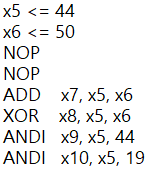
\includegraphics[width=0.2\textwidth]{sec3/images/test1.png}
	\caption{testing ALU and Register File}
	\label{fig:test1}
\end{figure}
The first instructions initialise registers x5 and x6 to two known values, then two NOPs are inserted to avoid data hazard and finally several arithmetic operations are performed and the results saved in registers. As can be seen from \todo{insert figure}, in registers x7, x8, x9 and x10 there are respectively sum, bitwise XOR and AND immediate once with an identical data and once with a different data.\\
It can be seen that all control signals are correctly synchronised and data is written to the Register File.